\documentclass{beamer}
\usetheme{Singapore}
\setbeamertemplate{navigation symbols}{}
\usepackage[utf8x]{inputenc}
\usepackage[light]{antpolt} % Provides awesome font
\usepackage{soul}	% Provides \st{} command
\usepackage{changepage}
\usepackage{tikz}
\usepackage{bm}
\usepackage[all]{xy}
\newcommand{\game}[6]{\begin{align*}\begin{array}{ccccccc} \text{I} & #1 && #3 && #5\\ \text{II} && #2 && #4 && #6 \end{array}\end{align*}}

\title[Determinacy]{Determinacy of games}
\author{Dan Saattrup Nielsen}
\date{November 25, 2016}

\begin{document}

{\setbeamertemplate{background canvas}{\tikz[remember picture,overlay,shift={(current page.center)}]\node[opacity=0.7] at (4.5,-4) {
\includegraphics[scale=0.15]{UoBlogo.png}};}

\begin{frame}
	\maketitle
\end{frame}}

\begin{frame}{The plan}
	\begin{itemize}
		\item\pause (Loose) introduction to games and determinacy
		\item\pause Consequences of determinacy
		\item\pause Which games \textit{are} determined?
		\item\pause A bird's eye view
	\end{itemize}
\end{frame}

\begin{frame}{Games}
	\begin{center}
		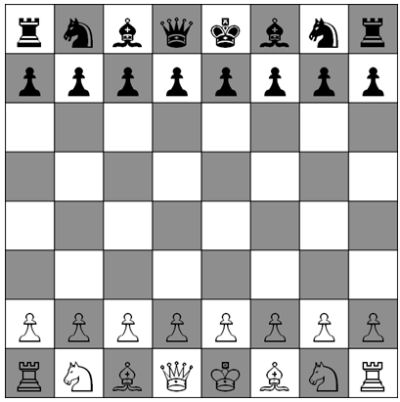
\includegraphics[scale=0.45]{chess.jpg}
	\end{center}
\end{frame}

\begin{frame}{Games}
	\begin{center}
		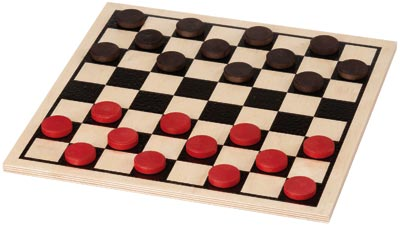
\includegraphics[scale=0.5]{checkers.jpg}
	\end{center}
\end{frame}

\begin{frame}{Games}
	\begin{center}
		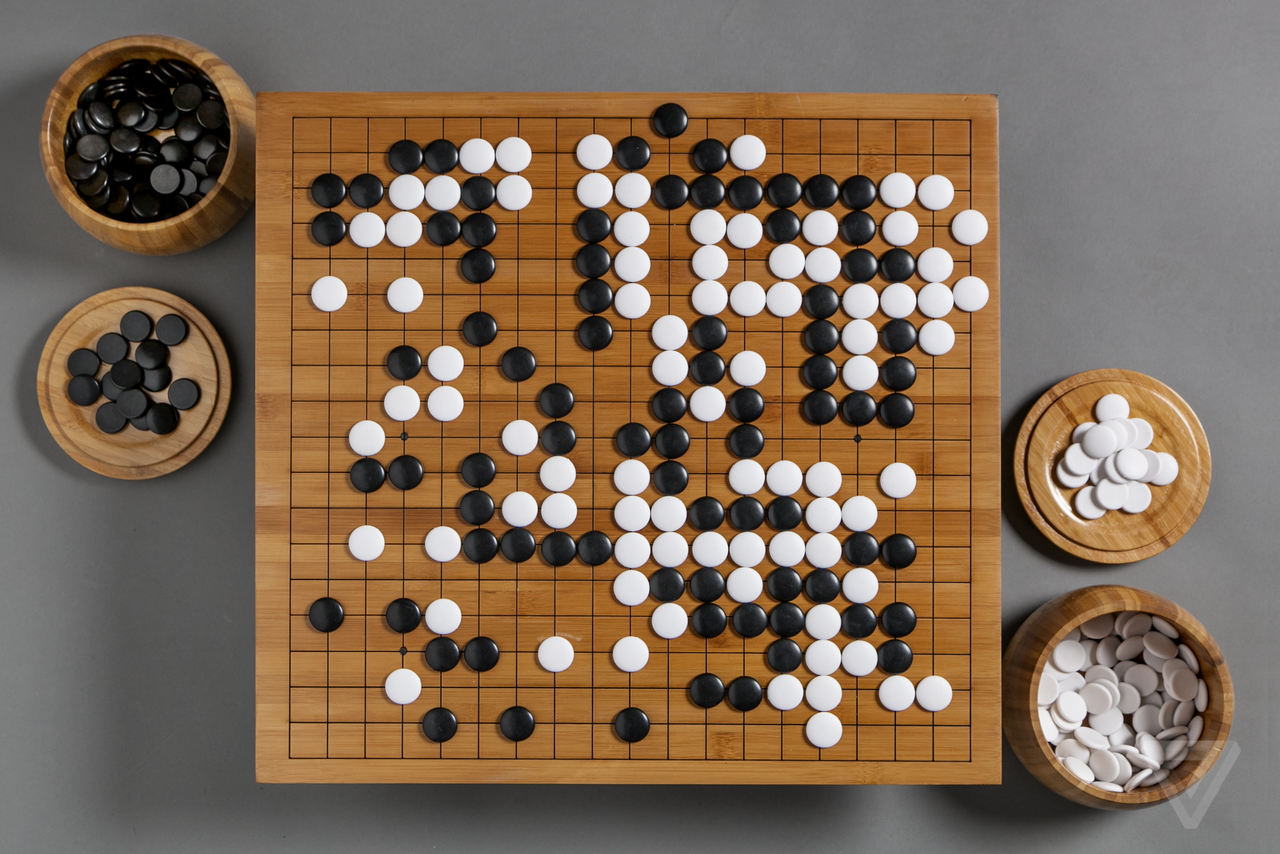
\includegraphics[scale=0.23]{go.png}
	\end{center}
\end{frame}

\begin{frame}{Games}
	Key properties:
	\begin{itemize}
		\item\pause 2 players
		\item\pause Perfect information
		\item\pause No draws
		\item\pause Finite
	\end{itemize}
\end{frame}

\begin{frame}{Winning strategies}
	Say $A$ is the set of winning moves for player I.\vspace{0.3cm}
 
	\only<1-2>{\onslide<2>Then player I has a \textcolor{red}{winning strategy} if
	\begin{align*}
		\exists x_0\in\omega\forall x_1\in\omega\cdots Qx_n\in\omega(\vec x\in A)
	\end{align*}}

	\only<3>{Then player \textcolor{red}{II} has a winning strategy if
	\begin{align*}
		\textcolor{red}{\forall} x_0\in\omega\textcolor{red}{\exists} x_1\in\omega\cdots Qx_n\in\omega(\vec x\ \textcolor{red}{\notin}\ A)
	\end{align*}}

	\only<4->{Then the game is \textcolor{red}{determined} if
		\begin{align*}
			&\lnot\exists x_0\in\omega\forall x_1\in\omega\cdots Qx_n\in\omega(\vec x\in A)\\
			\equiv&\forall x_0\in\omega\exists x_1\in\omega\cdots Qx_n\in\omega(\vec x\notin A)
		\end{align*}}
\end{frame}

\begin{frame}{Switching focus}
	Key properties:
	\begin{itemize}
		\item 2 players
		\item Perfect information
		\item No draws
		\item \only<1>{Finite}\only<2->{\st{Finite}}
		\item<3> Infinite
	\end{itemize}
\end{frame}


\begin{frame}{Winning strategies}
	Say $A$ is the set of winning moves for player I.\vspace{0.3cm}
 
	Then the game is \textcolor{red}{determined} if
		\only<1>{\begin{align*}
			\lnot\exists x_0\in\omega\forall x_1\in\omega\cdots(\vec x\in A)\equiv\forall x_0\in\omega\exists x_1\in\omega\cdots(\vec x\notin A)
		\end{align*}}
		\only<2->{\begin{align*}
			\lnot\Game^{\exists}\vec x(\vec x\in A)\equiv\Game^{\forall}\vec x(\vec x\notin A)
		\end{align*}}

	\onslide<3-> We can identify the set of all such sequences $\vec x$ with the reals.
\end{frame}

\begin{frame}{Consequence of determinacy}
	\pause\begin{block}{The Continuum Hypothesis ($\operatorname{CH}$)}
		Every infinite subset of the reals is either equinumerous with the integers or the reals.
	\end{block}

	\only<3>{\begin{block}{The Davis Game}
		Let $A$ be a set of reals, $s_i$ finite $0-1$ sequences and $x_i\in\{0,1\}$. Then the \textcolor{red}{Davis game} $\mathcal{G}(A)$ is played as
		\game{s_0}{x_0}{s_1}{x_1}{\cdots}{\cdots}

		Player I wins iff $s_0\widehat{\ }\left<x_0\right>\widehat{\ }s_1\widehat{\ }\cdots\in A$.
	\end{block}}

	\only<4>{\begin{block}{Theorem (Davis 1964)}
		If $\mathcal{G}(A)$ is determined then $\operatorname{CH}$ holds for $A$.$\hfill\dashv$
	\end{block}}
\end{frame}

\begin{frame}{Determinacy and choice}
	\pause\begin{block}{Theorem (AC)}
		There is an undetermined game.\vspace{0.3cm}
	\end{block}

	\pause \small{\textit{(Proof on board)}}
\end{frame}

\begin{frame}{Projective sets}

	We define the \textcolor<1-4>{red}{projective formulas} as:
	\begin{itemize}
		\item\pause $\varphi$ is $\Sigma^1_0$ if $\varphi\equiv\exists n\in\omega:\psi(n)$ for some $\psi$ having only quantifiers bounded by a finite set
		\item\pause $\varphi$ is $\Pi^1_n$ if $\varphi\equiv\lnot\psi$ for $\psi$ being $\Sigma^1_n$
		\item\pause $\varphi$ is $\Sigma^1_{n+1}$ if $\varphi\equiv\exists x\in\mathbb R:\psi(x)$ for $\psi$ being $\Pi^1_n$\vspace{0.3cm}
	\end{itemize}

	\only<5>{We also have the \textcolor<5>{red}{relativised versions} $\Sigma^0_n(x)$ and $\Pi^0_n(x)$ for reals $x$, and say $\varphi$ is $\bm\Sigma^0_n$ if $\varphi$ is $\Sigma^0_n(x)$ for some real $x$.}

	\only<6->{\begin{center}\xymatrix@R=3mm@C=5mm{
  & \textcolor<7-8>{red}{\bm\Sigma^1_0}\ar@{^{(}->}[dr] && \bm\Sigma^1_1\ar@{^{(}->}[dr] && \bm\Sigma^1_2\\
  \textcolor<8>{red}{\bm\Delta^1_0}\ar@{^{(}->}[ur]\ar@{^{(}->}[dr] && \textcolor<9>{red}{\bm\Delta^1_1}\ar@{^{(}->}[ur]\ar@{^{(}->}[dr] && \bm\Delta^1_2\ar@{^{(}->}[ur]\ar@{^{(}->}[dr] && \cdots\\
  & \textcolor<8>{red}{\bm\Pi^1_0}\ar@{^{(}->}[ur] && \textcolor<10>{red}{\bm\Pi^1_1}\ar@{^{(}->}[ur] && \bm\Pi^1_2
}\end{center}}

\end{frame}

\begin{frame}{Projective determinacy}

\begin{center}\xymatrix@R=3mm@C=5mm{
  & \bm\Sigma^1_0\ar@{^{(}->}[dr] && \bm\Sigma^1_1\ar@{^{(}->}[dr] && \bm\Sigma^1_2\\
  \bm\Delta^1_0\ar@{^{(}->}[ur]\ar@{^{(}->}[dr] && \bm\Delta^1_1\ar@{^{(}->}[ur]\ar@{^{(}->}[dr] && \bm\Delta^1_2\ar@{^{(}->}[ur]\ar@{^{(}->}[dr] && \cdots\\
  & \bm\Pi^1_0\ar@{^{(}->}[ur] && \bm\Pi^1_1\ar@{^{(}->}[ur] && \bm\Pi^1_2
}\end{center}

  \textcolor<1>{red}{Projective determinacy (PD)}: Every projective set is determined.\vspace{0.3cm}

  \onslide<2>{\begin{block}{Theorem (Martin, Steel)}
    Large cardinals imply PD.$\hfill\dashv$
  \end{block}}

\end{frame}

\begin{frame}{A bird's eye view}

  \onslide<1->\textcolor<1>{red}{Note:} $A\subset\mathbb R$ is projective iff $A$ is definable in $\left<\mathcal P(\omega),\omega,\in,+,\cdot\right>$\vspace{0.3cm}

  \onslide<2->Woodin (2003): ``PD is the \textcolor<2>{red}{'correct'} axiom for the structure $\left<\mathcal P(\omega),\omega,\in,+,\cdot\right>$"\vspace{0.3cm}

  \onslide<3->\textcolor<3>{red}{Note:} $V\equiv\left<\mathcal P(\operatorname{On}),\operatorname{On},\in,+,\cdot\right>$\vspace{0.3cm}

  \onslide<4-> \textcolor<4>{red}{The next step:} Find the 'correct' axiom for $\left<\mathcal P(\omega_1),\omega_1,\in,+,\cdot\right>$\vspace{0.3cm}

  \onslide<5-> \textcolor<5>{red}{Note:} $\operatorname{CH}$ is definable in $\left<\mathcal P(\omega_1),\omega_1,\in,+,\cdot\right>$

	\onslide<6->\begin{block}{Theorem (Woodin)}
		No matter what 'correct' axiom we choose, $\operatorname{CH}$ will turn out false.
	\end{block}
  

\end{frame}

\begin{frame}
  \begin{center}
    \Large{Thank you!}
  \end{center}
\end{frame}

\end{document}
